%!TEX root=masterproef.tex

\chapter{IDP en een co\"operatief algoritme}
\label{appendix:idp-cooperation}

\citep{krontiris2009cooperative} beschrijft enerzijds een theoretisch model
voor het zgn. \emph{Intrusion Detection Problem} (IDP) en biedt anderzijds een
zeer praktisch algoritme om gedistribueerd tot een consensus te komen voor het
ontmaskeren van een kwaadwillige knoop in het netwerk.

\section{IDP}
\label{section:idp}

Het theoretische model beschrijft het IDP aan de hand van $S = \{ s_1, s_2,
\dots s_n \}$, de set van sensoren in het netwerk, $N(s)$, de verzameling van
buren van $s$ en $D(s)$, de set van knopen die door $s$ verdacht worden. Indien
$|D(s)| = 1$, is de aanvaller ge\"identificeerd. Verder worden enkele
predicaten gedefinieerd als volgt:

\begin{subequations}
\begin{equation} \label{eq:honest}
honest(s) \iff \neg source(s)
\end{equation}
\begin{equation} \label{eq:expose}
expose_s(q) \iff D(s) = \{ q \}
\end{equation}
\begin{equation} \label{eq:alerted}
A(s) \iff D(s) \not= \{\}
\end{equation}
\begin{equation} \label{eq:alerted-neighbours}
AN(s) = \{ t | A(t) \wedge t \in N(s) \}
\end{equation}
\begin{equation} \label{eq:alerted-useful-neighbours}
\tilde{AN}(q,s) = AN(q) \backslash \{s\}
\end{equation}
\end{subequations}
  
\ref{eq:honest} definieert een eerlijke knoop (\emph{honest}) en de aanvaller
als de oorsprong van de aanval (\emph{source}). \ref{eq:expose} stelt dat een
knoop $s$ een andere knoop $q$ kan ontmaskeren (\emph{expose}) als de
aanvaller, indien de verzameling van knopen die door $s$ verdacht worden alleen
$q$ bevat. \ref{eq:alerted} verzamelt alle knopen die andere knopen verdenken,
ook wel gealarmeerde knopen genoemd. Indien deze knopen buren zijn van $s$, dan
bestaat de verzameling van gealarmeerde buren volgens
\ref{eq:alerted-neighbours}. \ref{eq:alerted-useful-neighbours} tot slot
definieert de verzameling van gealarmeerde buren van $q$ die nuttig zijn voor
$s$.

Het IDP wordt vervolgens gedefinieerd als het vinden van een algoritme dat
voldoet aan de eigenschappen van correctheid (\ref{eq:idp-correctness}) en
eindigheid: bij een aanval zullen na een tijd alle eerlijke knopen in de
gealarmeerde set een knoop verdenken.

\begin{equation} \label{eq:idp-correctness}
\forall s \in S : honest(s) \wedge expose_s(s') \implies A(s) \wedge source(s')
\end{equation}

Twee condities worden voorgesteld: de \emph{Intrusion Detection Condition}
(IDC) en de \emph{Neighbourhood Conditions} (NC). Indien aan minstens \'e\'en
van deze condities voldaan is, is het IDP oplosbaar. De IDC stelt dat geen
enkele andere knoop een zelfde gealarmeerde buurt kan hebben als de aanvaller:

\begin{equation} \label{eq:idc}
\forall p,q \in S : source(q) \implies \tilde{AN}(p,q) \not= \tilde{AN}(q,p)
\end{equation}

De NC worden beschreven door ``\emph{alle buren van een aanvaller zijn
gealarmeerd}'' ($NC_1$) en ``\emph{indien twee of meer knopen verdacht zijn door
een meerderheid van knopen, hebben de eerlijke knopen niet-gealarmeerde buren}''
($NC_2$).

Figuur \ref{fig:idp-examples} illustreert het IDP en toepassing van IDC en NC
aan de hand van enkele voorbeelden:

\begin{figure}[ht]
\centering
\begin{subfigure}{.49\textwidth}
  \centering
  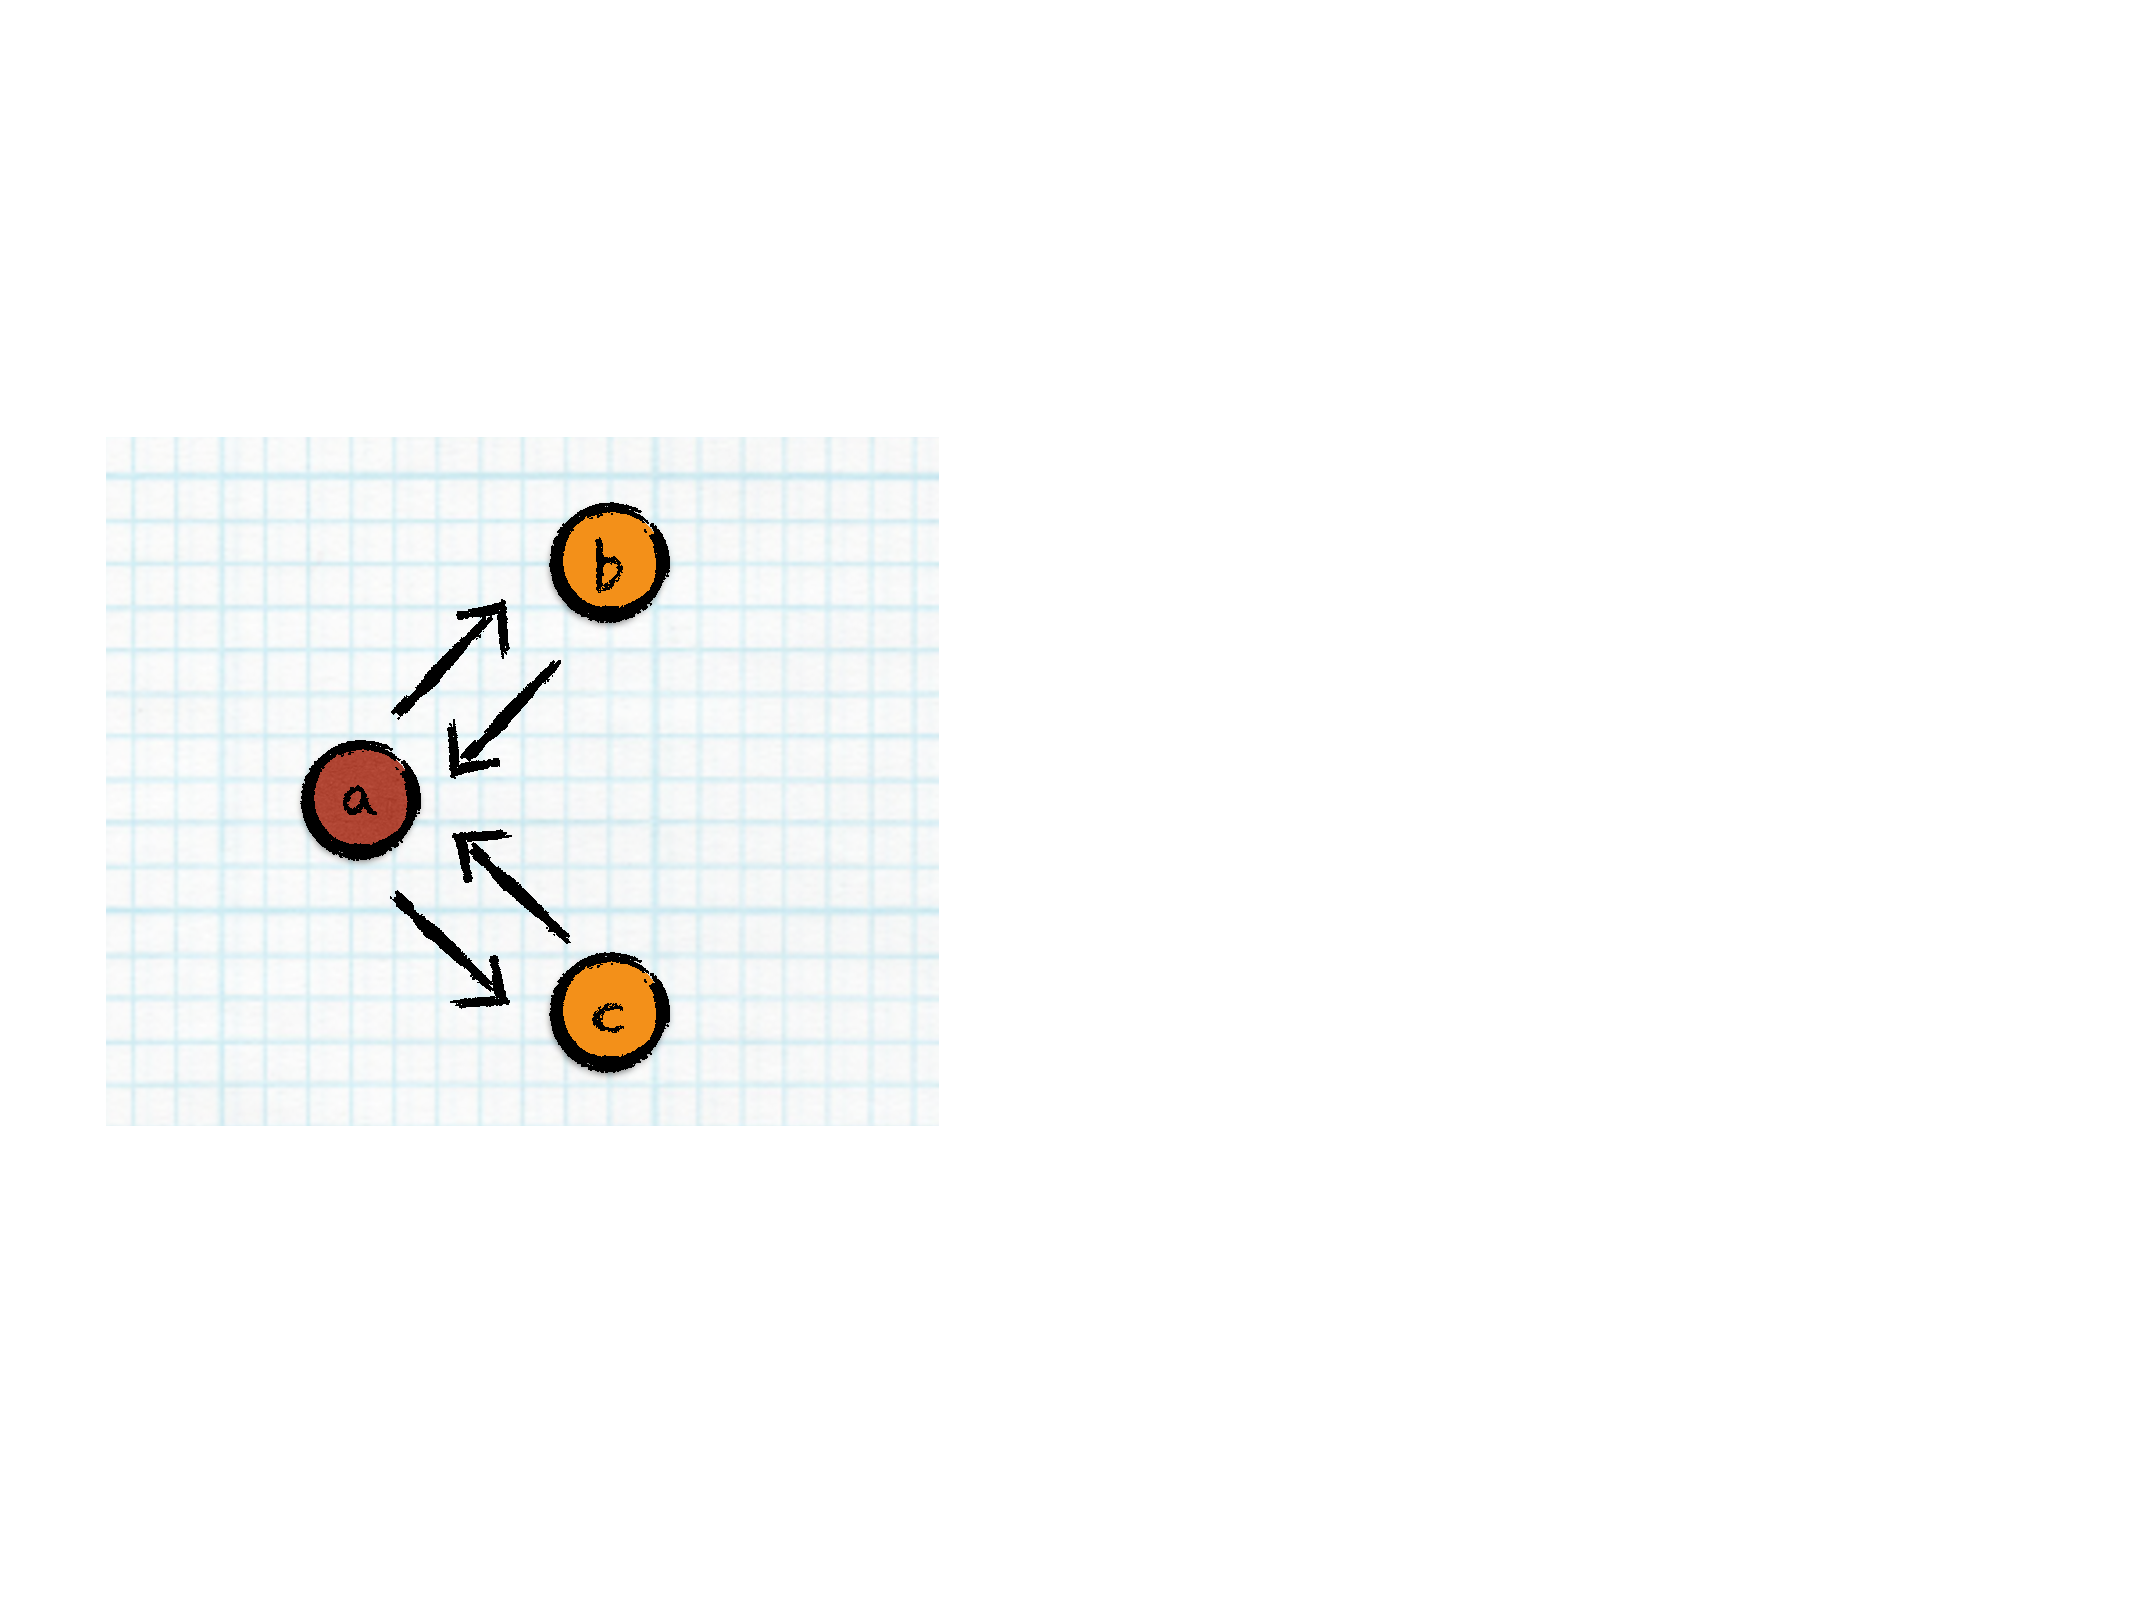
\includegraphics[width=.8\linewidth]{./resources/idp-nc-s1.pdf}
  \caption{}
  \label{fig:idp-examples-1}
\end{subfigure}
\begin{subfigure}{.49\textwidth}
  \centering
  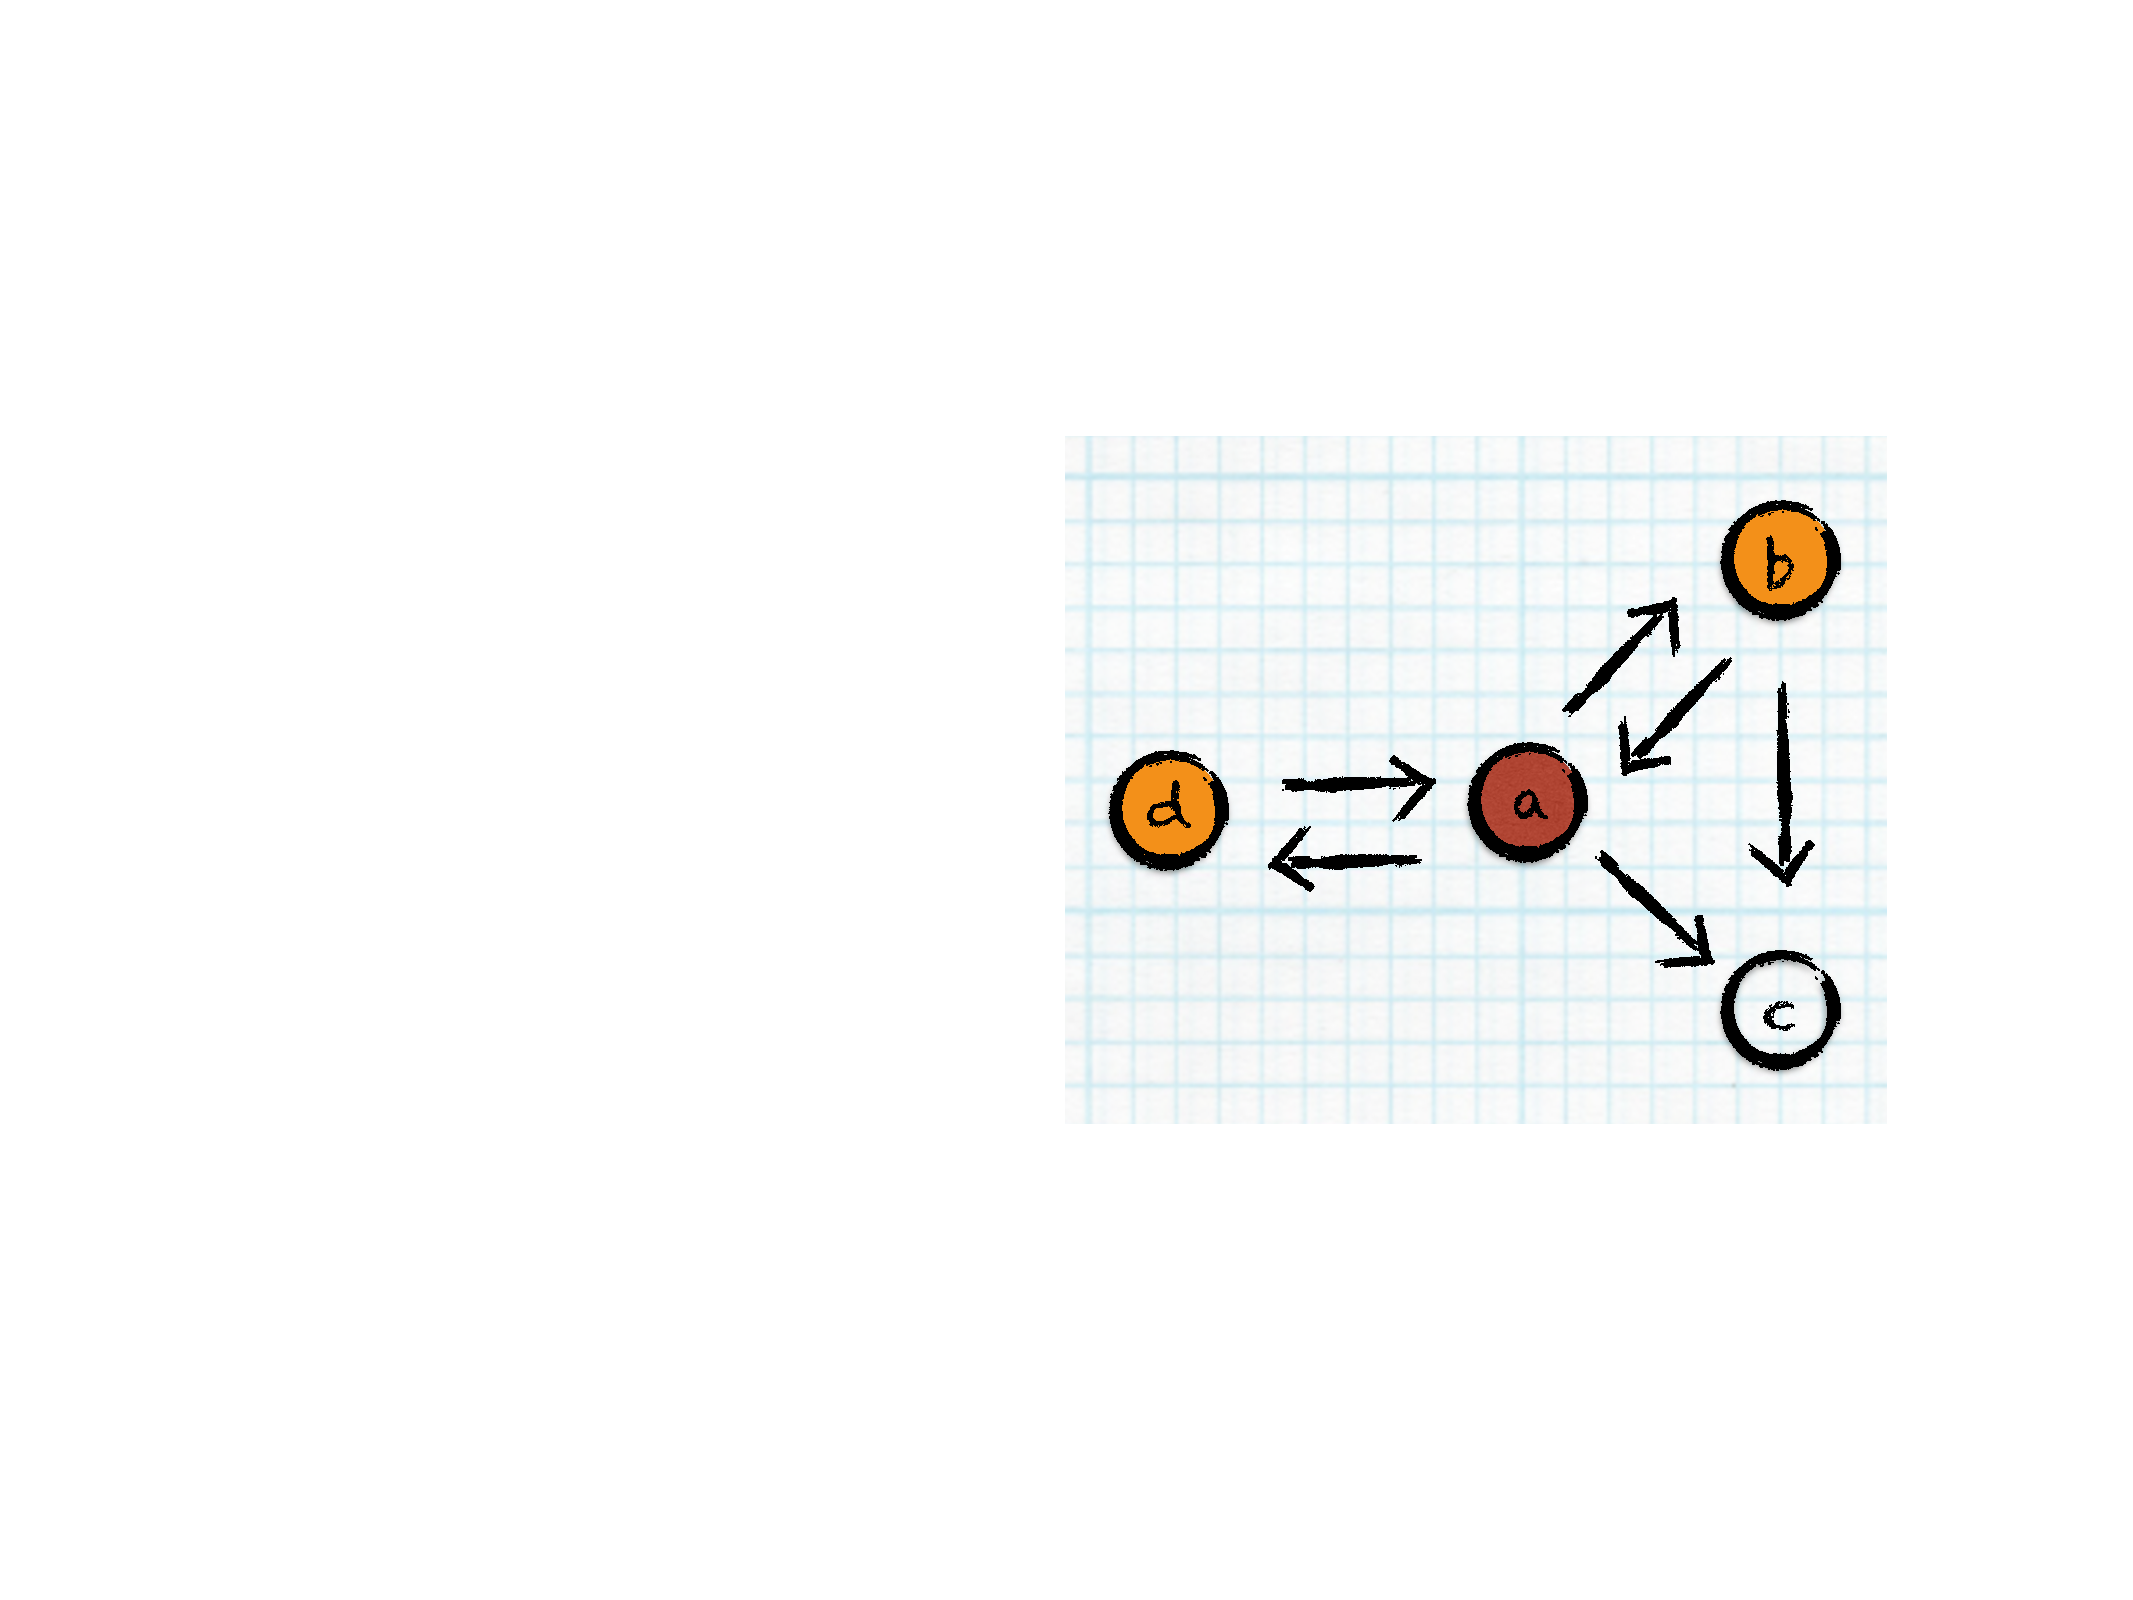
\includegraphics[width=.8\linewidth]{./resources/idp-nc-s2.pdf}
  \caption{}
  \label{fig:idp-examples-2}
\end{subfigure}
\caption[Voorbeelden van de toepassing van IDC en NC]{Voorbeelden van de
toepassing van IDC en NC: Rode knopen zijn aanvallers, gekleurde knopen zijn
gealarmeerd. $x \rightarrow y$ betekent dat knoop $x$ knoop y verdenkt}
\label{fig:idp-examples}
\end{figure}

De situatie in figuur \ref{fig:idp-examples-1} voldoet niet aan de IDC omdat
$\tilde{AN}(a,b) = \{c\} = \tilde{AN}(b,a)$. Maar in dit geval is wel voldaan
aan beide NC. Het IDP kan in dit geval opgelost worden aan de hand van een
deterministisch algoritme. Omdat er slechts \'e\'en knoop het hoogste aantal
verdenkingen op zijn naam heeft staan, kunnen knopen $b$ en $c$ eenvoudig
beslissen dat knoop $a$ de aanvaller is.

Figuur \ref{fig:idp-examples-2} toont een situatie waar de IDC wel voldaan is
want $\tilde{AN}(a,b) = \{d\} \not= \tilde{AN}(b,a) = \{\}$. Er zijn nu echter
twee knopen met een meerderheid aan verdenkingen: $a$ en $c$. Vanuit het
standpunt van knoop $b$ moet dus knoop $a$ of knoop $d$ valse aantijgingen
verspreiden. Als \'e\'en van deze knopen de aanvaller is, dan moet
$\tilde{AN}(a,d) \not= \tilde{AN}(d,a)$, anders is niet voldaan aan de IDC. Dit
impliceert tevens dat $\exists x : A(x) \wedge ( x \not\in N(a) \vee x \not\in
N(d) )$, ofwel dat er een knoop bestaat die gealarmeerd is, maar geen buur is
van de andere eerlijke knoop van de twee verdachte knopen. In dit geval zijn
knopen $b$ en $d$ inderdaad geen buren, maar beide verdenken knoop $a$.

\section{Algoritme}
\label{section:cooperation-algorithm}

Naast een theoretisch model, introduceren \citep{krontiris2009cooperative}
tevens een algoritme dat kan dienen als raamwerk voor co\"operatieve
inbraakdetectie. Het algoritme bestaat uit vier tot vijf fasen: initialisatie,
stemming, publicatie van gebruikte sleutels, ontmaskeren van de aanvaller en
optioneel het inroepen van informatie uit de externe kring. Het is in essentie
een implementatie van het Guy Fawkes-protocol, beschreven in
\citep{anderson1998new}, dat toelaat om een reeks van berichten te authenticeren
op basis van \'e\'en initieel gedeelde sleutel.

Tijdens de initialisatiefase krijgt elke knoop een unieke sleutel, $K_l$. Aan
de hand van deze sleutel wordt een \'e\'enrichtingsketting van lengte $l$
gemaakt van sleutels door bv. SHA1-hashing \citep{rfc:3174} toe te passen:
$\{K_0, K_1,\dots K_{l-1}\}$ waarbij $\forall k \in [1..l] : K_{k-1} =
SHA1(K_k)$. Daarnaast worden ook naburige knopen gezocht tot twee knopen ver en
wordt sleutel $K_0$ gecommuniceerd aan al deze buren. De initialisatiefase
wordt verondersteld te gebeuren zonder mogelijkheid tot inbraken.

Tijdens de stemming brengen alle knopen een stem uit van de vorm $m_v(s),$ $
MAC_{K_j}(m_v(s))$. $m_v(s)$ bestaat uit een lijst van knopen die door knoop
$s$ beschouwd worden als mogelijke aanvallers, of uitgedrukt aan de hand van
het IDP: $m_v(s) = D(s)$. De $MAC_{K_j}()$ functie is een zgn. \emph{Message
Authentication Code} \citep{rfc:2104} en wordt meestal berekend door het
toepassen van een \'e\'enrichtings-hashfunctie op de boodschap. Typisch wordt
er aan de boodschap een unieke, wederzijds gekende identificatie toegevoegd,
zodat de ontvanger van een boodschap deze handtekening ook kan berekenen en
vergelijken met het origineel. In dit geval wordt $K_j$ gebruikt, waarbij $j$
de volgende indexwaarde krijgt uit lijst van beschikbare sleutels.

Een dergelijke boodschap kan op het ogenblik van verzending door geen enkele
andere knoop gevalideerd worden. De enige sleutel die zij tot op dat ogenblik
kennen is de vorige en deze is net het resultaat van een SHA1-operatie op de
volgende. Dit betekent dat ook een mogelijke aanvaller niet in staat is om de
boodschap te wijzigen.

Pas wanneer de knopen elkaars stemmen hebben ontvangen, wordt de gebruikte
sleutel vrijgegeven in de publicatiefase. Op dit ogenblik kunnen de knopen de
eerder verstuurde stemmen valideren. Ze kunnen eerst controleren of de
gepubliceerde sleutel inderdaad de juiste is. Immers, door het toepassen van
SHA1 op deze sleutel ($K_j$), moeten zij de huidige gekende sleutel ($K_{j-1}$)
bekomen. Na validatie van de nieuwe sleutel, kan ook de boodschap gevalideerd
worden.

Nu alle knopen de stemmen van alle knopen ontvangen hebben en zeker zijn dat de
stemmen authentiek zijn, kan met \'e\'enzelfde algoritme door alle knopen de
aanvaller bepaald worden tijdens de ontmaskering.

Het is echter mogelijk dat er meerdere knopen zijn met eenzelfde aantal
stemmen, wat overeenkomt met een gelijke samenstelling van gealarmeerde buren,
wanneer de IDC niet kan gerealiseerd worden. Onder voorbehoud dat aan de NC wel
voldaan wordt, kan door het inroepen van de niet-gealarmeerde buren van de
gealarmeerde knopen, de zgn. externe kring, een oplossing bekomen worden. Deze
zullen op hun beurt nagaan of de knopen die verdacht worden, buren zijn en dan
aangeven dat zij hen \emph{niet} verdenken. Aan de hand van deze informatie
kunnen de gealarmeerde knopen hun beslissing staven.
